\documentclass[]{article}
\usepackage{lmodern}
\usepackage{amssymb,amsmath}
\usepackage{ifxetex,ifluatex}
\usepackage{fixltx2e} % provides \textsubscript
\ifnum 0\ifxetex 1\fi\ifluatex 1\fi=0 % if pdftex
  \usepackage[T1]{fontenc}
  \usepackage[utf8]{inputenc}
\else % if luatex or xelatex
  \ifxetex
    \usepackage{mathspec}
    \usepackage{xltxtra,xunicode}
  \else
    \usepackage{fontspec}
  \fi
  \defaultfontfeatures{Mapping=tex-text,Scale=MatchLowercase}
  \newcommand{\euro}{€}
\fi
% use upquote if available, for straight quotes in verbatim environments
\IfFileExists{upquote.sty}{\usepackage{upquote}}{}
% use microtype if available
\IfFileExists{microtype.sty}{%
\usepackage{microtype}
\UseMicrotypeSet[protrusion]{basicmath} % disable protrusion for tt fonts
}{}
\usepackage[margin=1in]{geometry}
\usepackage{longtable,booktabs}
\usepackage{graphicx}
\makeatletter
\def\maxwidth{\ifdim\Gin@nat@width>\linewidth\linewidth\else\Gin@nat@width\fi}
\def\maxheight{\ifdim\Gin@nat@height>\textheight\textheight\else\Gin@nat@height\fi}
\makeatother
% Scale images if necessary, so that they will not overflow the page
% margins by default, and it is still possible to overwrite the defaults
% using explicit options in \includegraphics[width, height, ...]{}
\setkeys{Gin}{width=\maxwidth,height=\maxheight,keepaspectratio}
\ifxetex
  \usepackage[setpagesize=false, % page size defined by xetex
              unicode=false, % unicode breaks when used with xetex
              xetex]{hyperref}
\else
  \usepackage[unicode=true]{hyperref}
\fi
\hypersetup{breaklinks=true,
            bookmarks=true,
            pdfauthor={Heather E. Wheeler1, Nicholas Knoblauch2, GTEx Consortium, Nancy J. Cox3, Dan L. Nicolae1, Hae Kyung Im1},
            pdftitle={Genetic architecture of transcriptome regulation and orthogonal tissue decompositon},
            colorlinks=true,
            citecolor=blue,
            urlcolor=blue,
            linkcolor=magenta,
            pdfborder={0 0 0}}
\urlstyle{same}  % don't use monospace font for urls
\setlength{\parindent}{0pt}
\setlength{\parskip}{6pt plus 2pt minus 1pt}
\setlength{\emergencystretch}{3em}  % prevent overfull lines
\setcounter{secnumdepth}{0}

%%% Use protect on footnotes to avoid problems with footnotes in titles
\let\rmarkdownfootnote\footnote%
\def\footnote{\protect\rmarkdownfootnote}

%%% Change title format to be more compact
\usepackage{titling}

% Create subtitle command for use in maketitle
\newcommand{\subtitle}[1]{
  \posttitle{
    \begin{center}\large#1\end{center}
    }
}

\setlength{\droptitle}{-2em}
  \title{Genetic architecture of transcriptome regulation and orthogonal tissue
decompositon}
  \pretitle{\vspace{\droptitle}\centering\huge}
  \posttitle{\par}
  \author{Heather E. Wheeler\textsuperscript{1}, Nicholas
Knoblauch\textsuperscript{2}, GTEx Consortium, Nancy J.
Cox\textsuperscript{3}, Dan L. Nicolae\textsuperscript{1}, Hae Kyung
Im\textsuperscript{1}}
  \preauthor{\centering\large\emph}
  \postauthor{\par}
  \predate{\centering\large\emph}
  \postdate{\par}
  \date{2015-05-26 09:50:46 \textsuperscript{1}Department of Medicine,
University of Chicago, \textsuperscript{2}Committee on Genetics,
Genomics, and Systems Biology, University of Chicago,
\textsuperscript{3}Division of Genetic Medicine, Vanderbilt University}



\begin{document}

\maketitle


\section{Abstract}\label{abstract}

\emph{Lorem ipsum dolor sit amet, est ad doctus eligendi scriptorem. Mel
erat falli ut. Feugiat legendos adipisci vix at, usu at laoreet
argumentum suscipiantur. An eos adhuc aliquip scriptorem, te adhuc dolor
liberavisse sea. Ponderum vivendum te nec, id agam brute disputando
mei.}

\section{Introduction}\label{introduction}

cite Kruglyak review, Price PGen 11, Wright NatGen 14

\section{Results}\label{results}

\subsection{Local genetic variation explains a large proportion of gene
expression
variance}\label{local-genetic-variation-explains-a-large-proportion-of-gene-expression-variance}

We estimated the heritability of gene expression in whole blood from the
Depression Genes and Networks (DGN) cohort (n=922) {[}1{]} using a
mixed-effects model (see Methods) and calculated variances using
restricted maximum likelihood as implemented in GCTA {[}2{]}. We fit a
joint model with a local and a global genetic relationship matrix (GRM).
The local GRM was derived from SNPs within 1 Mb of each gene and the
global GRM was derived from SNPs that are located on non-gene
chromosomes and are eQTLs in the Framingham Heart Study (FHS) cohort
(n=5257, FDR \textless{} 0.05) {[}3{]}. The mean local
h\textsuperscript{2} was 0.130 and 54.6\% of genes had a positive 95\%
confidence interval (CI), while the mean global h\textsuperscript{2} was
0.076 and just 4.2\% of genes had a positive CI (Fig 1). The maximum
local h\textsuperscript{2} was 0.93 with a standard error (SE) of 0.009
while the maximum global h\textsuperscript{2} was 0.91 with a SE of
0.16. Similar results were observed for the 1194 genes with
\emph{trans}-eQTLs (FHS FDR \textless{} 0.05) when the global GRM was
limited to known \emph{trans}-eQTLs (Fig 2). That is, the mean local
h\textsuperscript{2} was 0.133 and 61.3\% of genes had a positive 95\%
confidence interval (CI), while the mean \emph{trans}
h\textsuperscript{2} was just 0.021 and 4.2\% of genes tested had a
positive CI.

\subsection{Cross-tissue and tissue-specific gene expression by
orthogonal tissue
decomposition}\label{cross-tissue-and-tissue-specific-gene-expression-by-orthogonal-tissue-decomposition}

In order to better understand the context specificity of gene expression
regulation, we developed a method called orthogonal tissue decomposition
(OTD), which uses a mixed effects model to generate cross-tissue and
tissue-specific gene expression levels (see Methods). Using a marginal
model with just the local GRM, we estimated the local
h\textsuperscript{2} of cross-tissue gene expression and tissue-specific
gene expression in the nine tissues with the most samples. The
cross-tissue heritabilities were larger and the standard errors were
smaller than the tissue-specific estimates (Fig 3). The percentage of
h\textsuperscript{2} estimates with positive CIs was much larger for
cross-tissue expression (17.3\%) than the tissue-specific expressions
(all less than 3\%, Fig 4).

We also compared the cross-tissue h\textsuperscript{2} from the OTD to
h\textsuperscript{2} estimates from the pre-OTD measures of gene
expression in each of the nine tissues, which we term tissue-wide
expression. Again, the cross-tissue heritabilities were larger and the
standard errors were smaller than the tissue-wide estimates (Fig 5),
though less striking than the tissue-specific comparison. The percentage
of tissue-wide h\textsuperscript{2} estimates with positive CIs ranged
from 4.4-8.6\% and thus were all larger than the tissue-specific postive
CI percentages, but smaller than the cross-tissue percentage (Fig 6).

\subsection{The effect of local genetic variation on gene expression is
sparse rather than
polygenic}\label{the-effect-of-local-genetic-variation-on-gene-expression-is-sparse-rather-than-polygenic}

We performed 10-fold cross-validation using the elastic net to test the
predictive performance of local SNPs for gene expression across a range
of mixing parameters, \(\alpha\). The \(\alpha\) that gives the largest
cross-validation R\textsuperscript{2} informs the sparsity of each gene
expression trait. That is, at one extreme, if the optimal \(\alpha=0\)
(equivalent to ridge regression), the gene expression trait is highly
polygenic, whereas if the optimal \(\alpha=1\) (equivalent to LASSO),
the trait is highly sparse. We found that for most gene expression
traits, the cross-validated R\textsuperscript{2} was suboptimal for
\(\alpha=0\) and \(\alpha=0.05\), but nearly identically optimal for
\(\alpha=0.5\) and \(\alpha=1\) in the DGN cohort (Fig 7). Therefore,
the effect of local genetic variation on gene expression is sparse
rather than polygenic.

\subsection{Citations}\label{citations}

The relationship was first described by Reference 4. However, there are
also opinions that the relationship is spurious {[}5{]}. We used R for
our calculations {[}6{]}, and we used package \texttt{knitcitations}
{[}7{]} to make the bibliography.

\section{Discussion}\label{discussion}

\begin{enumerate}
\def\labelenumi{\arabic{enumi}.}
\itemsep1pt\parskip0pt\parsep0pt
\item
  local + trans heritability (others have done this)
\item
  trans heritability estimates not reliable, proportion not reliable
\item
  orthogonal tissue decomposition
\item
  cross tissue + tissue specific heritability -- estimates higher and se
  lower for cross-tissue The tissue availability is unbalanced because
  of the difficulties of sample collection and the uneven quality of the
  tissues. Furthermore, by using a mixed effects model to create
  cross-tissue expression, we borrow information across tissues, which
  should increase our power to detect associations and achieve better
  predictive models.
\item
  elastic net mixing parameter (alpha) as measure of
  polygenicity/sparsity
\end{enumerate}

Future

\begin{enumerate}
\def\labelenumi{\arabic{enumi}.}
\itemsep1pt\parskip0pt\parsep0pt
\item
  simulation to show sparsity well represented by alpha
\item
  use number of PC's (computed using only local snps) that maximize
  prediction performance. This will count independent signals.
\item
  FHS heritability. could this improve trans heritability?
\end{enumerate}

\section{Methods}\label{methods}

\subsection{Genomic and Transcriptomic
Data}\label{genomic-and-transcriptomic-data}

\subsubsection{DGN Dataset}\label{dgn-dataset}

We obtained whole blood RNA-Seq and genome-wide genotype data for 922
individuals from the Depression Genes and Networks (DGN) cohort {[}1{]},
all of European ancestry. For our analyses, we used the HCP (hidden
covariates with prior) normalized gene-level expression data used for
the \emph{trans}-eQTL analysis in Battle et al. {[}1{]} and downloaded
from the NIMH repository. Approximately 650K SNPs (minor allele
frequency {[}MAF{]} \textgreater{} 0.05, Hardy-Weinberg Equilibrium {[}P
\textgreater{} 0.05{]}, non-ambiguous strand {[}no A/T or C/G SNPs{]})
comprised the input set of SNPs for imputation, which was performed on
the University of Michigan Imputation-Server
(\url{https://imputationserver.sph.umich.edu/start.html}) {[}8,9{]} with
the following parameters: 1000G Phase 1 v3 ShapeIt2 (no singletons)
reference panel, SHAPEIT phasing, and EUR population. Approximately 1.9M
non-ambiguous strand SNPs with MAF \textgreater{} 0.05, imputation
R\textsuperscript{2} \textgreater{} 0.8 and, to reduce computational
burden, inclusion in HapMap Phase II were retained for subsequent
analyses.

\subsubsection{GTEx Dataset}\label{gtex-dataset}

\subsection{Partitioning local and global heritability of gene
expression}\label{partitioning-local-and-global-heritability-of-gene-expression}

\subsection{Orthogonal tissue
decomposition}\label{orthogonal-tissue-decomposition}

We will use a mixed effects model to estimate these components and
enforce orthogonality of the components. This approach is an extension
of our method to develop an intrinsic growth phenotype13.

\subsection{Determining polygenicity versus sparsity using the elastic
net}\label{determining-polygenicity-versus-sparsity-using-the-elastic-net}

\subsection{Equations}\label{equations}

The deterministic part of the model is defined by this \textbf{in-line
equation} as \(\mu_i = \beta_0 + \beta_1x\), and the stochastic part by
the \textbf{centered equation}:

\[ \frac{1}{\sqrt{2\pi}\sigma}e^{-(x-\mu_i)^2/(2\sigma^2)} \]

\subsection{Tables}\label{tables}

\begin{longtable}[c]{@{}lrrrr@{}}
\caption{This is a GLM summary table.}\tabularnewline
\toprule
& Estimate & Std. Error & t value &
Pr(\textgreater{}\textbar{}t\textbar{})\tabularnewline
\midrule
\endfirsthead
\toprule
& Estimate & Std. Error & t value &
Pr(\textgreater{}\textbar{}t\textbar{})\tabularnewline
\midrule
\endhead
(Intercept) & 0.06 & 0.11 & 0.55 & 0.59\tabularnewline
x & 2.02 & 0.11 & 18.07 & 0.00\tabularnewline
\bottomrule
\end{longtable}

\section{Figures}\label{figures}

\begin{figure}[htbp]
\centering
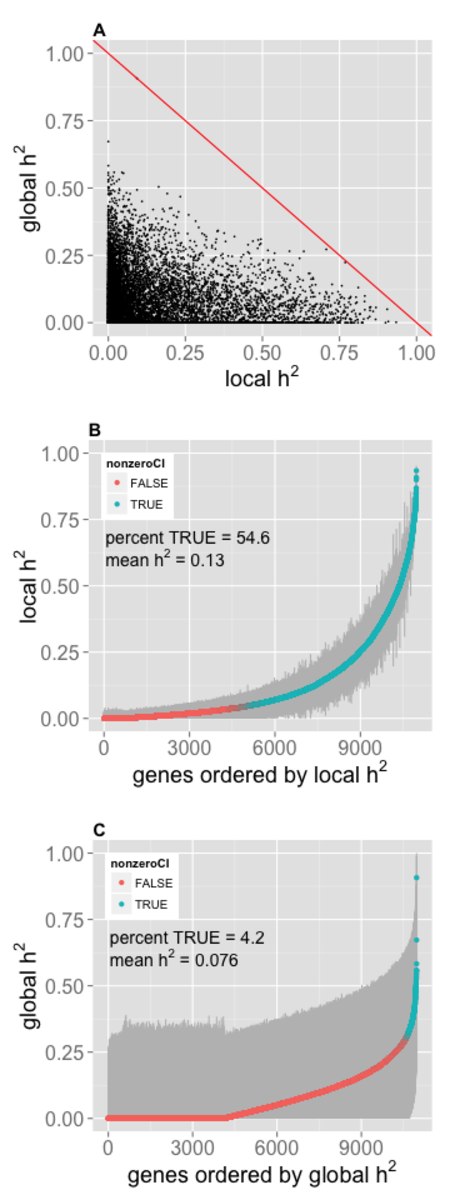
\includegraphics{GenArch_manuscript_files/figure-latex/jointH2-1.pdf}
\caption{DGN whole blood expression joint heritability
(h\textsuperscript{2}). Local (SNPs within 1 Mb of each gene) and global
(SNPs that are eQTLs in the Framingham Heart Study on other chromosomes
{[}FDR \textless{} 0.05{]}) h\textsuperscript{2} for gene expression
were jointly estimated. (\textbf{A}) Global h\textsuperscript{2}
compared to local h\textsuperscript{2} per gene. (\textbf{B}) Local and
(\textbf{C}) global gene expression h\textsuperscript{2} estimates
ordered by increasing h\textsuperscript{2}. The 95\% confidence interval
(CI) of each h\textsuperscript{2} estimate is in gray and genes with a
lower bound greater than zero are in blue.}
\end{figure}

\begin{figure}[htbp]
\centering
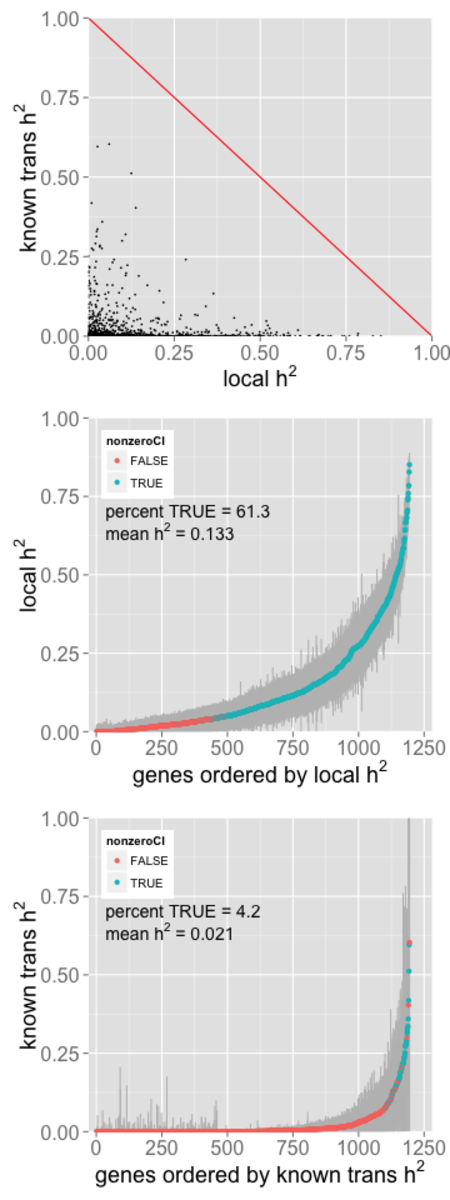
\includegraphics{GenArch_manuscript_files/figure-latex/transH2-1.pdf}
\caption{DGN whole blood expression joint heritability
(h\textsuperscript{2}) with known trans-eQTLs. Local (SNPs within 1 Mb
of each gene) and known trans (SNPs that are trans-eQTLs in the
Framingham Heart Study for each gene {[}FDR \textless{} 0.05{]})
h\textsuperscript{2} for gene expression were jointly estimated.
(\textbf{A}) Known trans h\textsuperscript{2} compared to local
h\textsuperscript{2} per gene. (\textbf{B}) Local and (\textbf{C}) known
trans gene expression h\textsuperscript{2} estimates ordered by
increasing h\textsuperscript{2}. The 95\% confidence interval (CI) of
each h\textsuperscript{2} estimate is in gray and genes with a lower
bound greater than zero are in blue.}
\end{figure}

\begin{figure}[htbp]
\centering
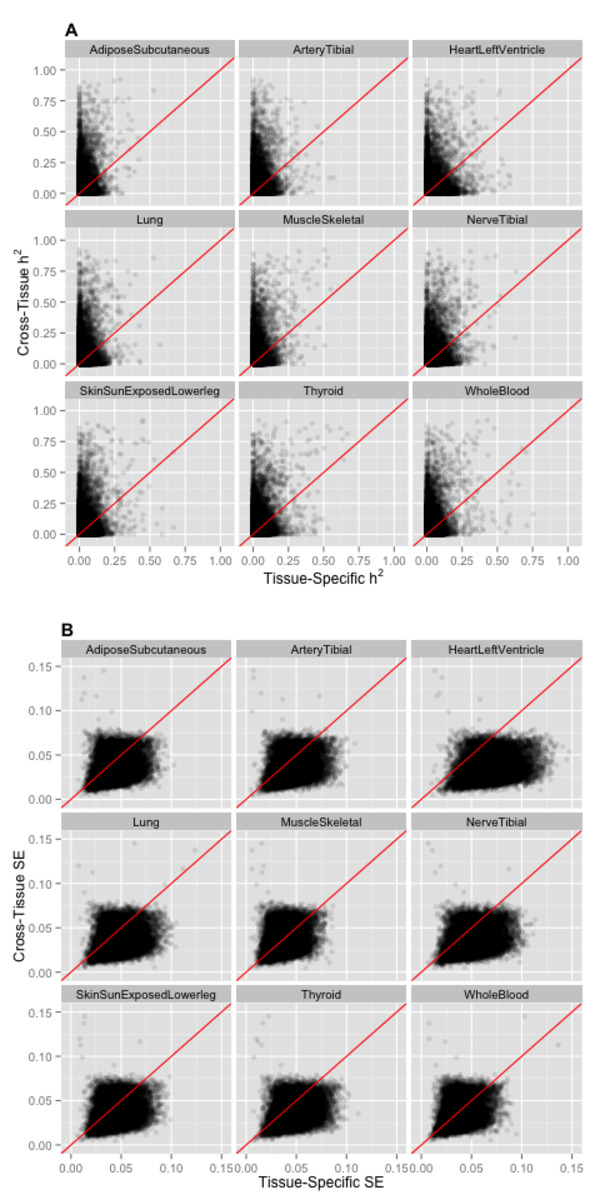
\includegraphics{GenArch_manuscript_files/figure-latex/TSotdH2SE-1.pdf}
\caption{Cross-tissue and tissue-specific comparison of heritability
(h\textsuperscript{2}, \textbf{A}) and standard error (SE, \textbf{B})
estimation. Cross-tissue local h\textsuperscript{2} is estimated using
the cross-tissue component (random effects) of the mixed effects model
for gene expression and SNPs within 1 Mb of each gene. Tissue-specifc
local h\textsuperscript{2} is estimated using the tissue-specific
component (residuals) of the mixed effects model for gene expression for
each respective tissue and SNPs within 1 Mb of each gene.}
\end{figure}

\begin{figure}[htbp]
\centering
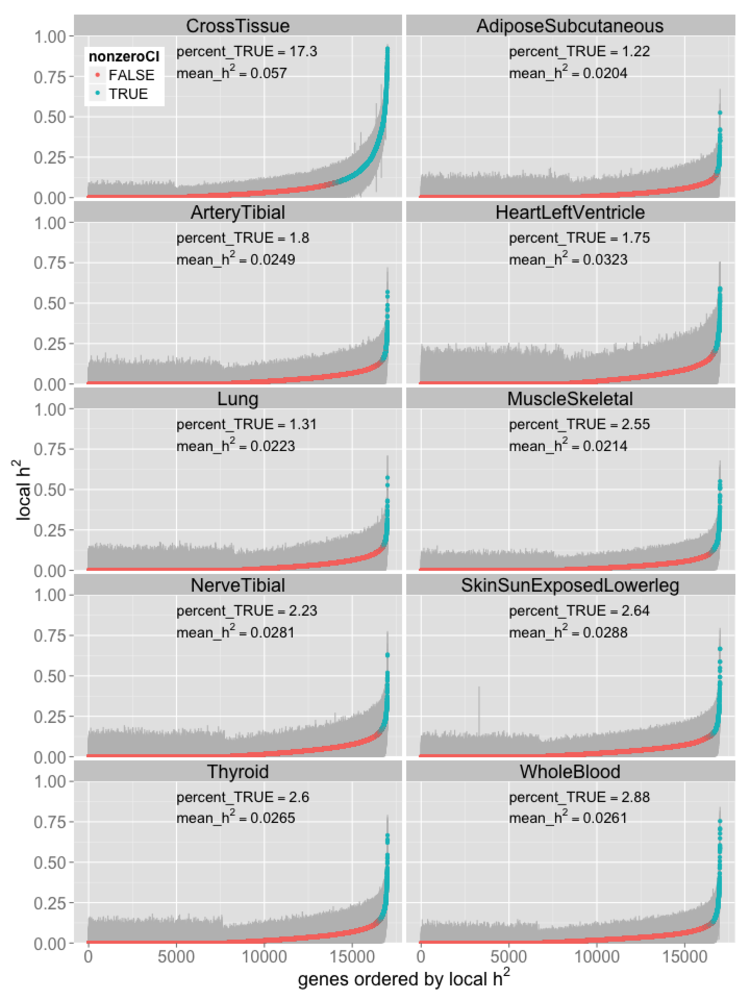
\includegraphics{GenArch_manuscript_files/figure-latex/otdTSh2-1.pdf}
\caption{Cross-tissue heritability (h\textsuperscript{2}) compared to
tissue-specific h\textsuperscript{2}. Cross-tissue local
h\textsuperscript{2} is estimated using the cross-tissue component
(random effects) of the mixed effects model for gene expression and SNPs
within 1 Mb of each gene. Tissue-specifc local h\textsuperscript{2} is
estimated using the tissue-specific component (residuals) of the mixed
effects model for gene expression for each respective tissue and SNPs
within 1 Mb of each gene.}
\end{figure}

\begin{figure}[htbp]
\centering
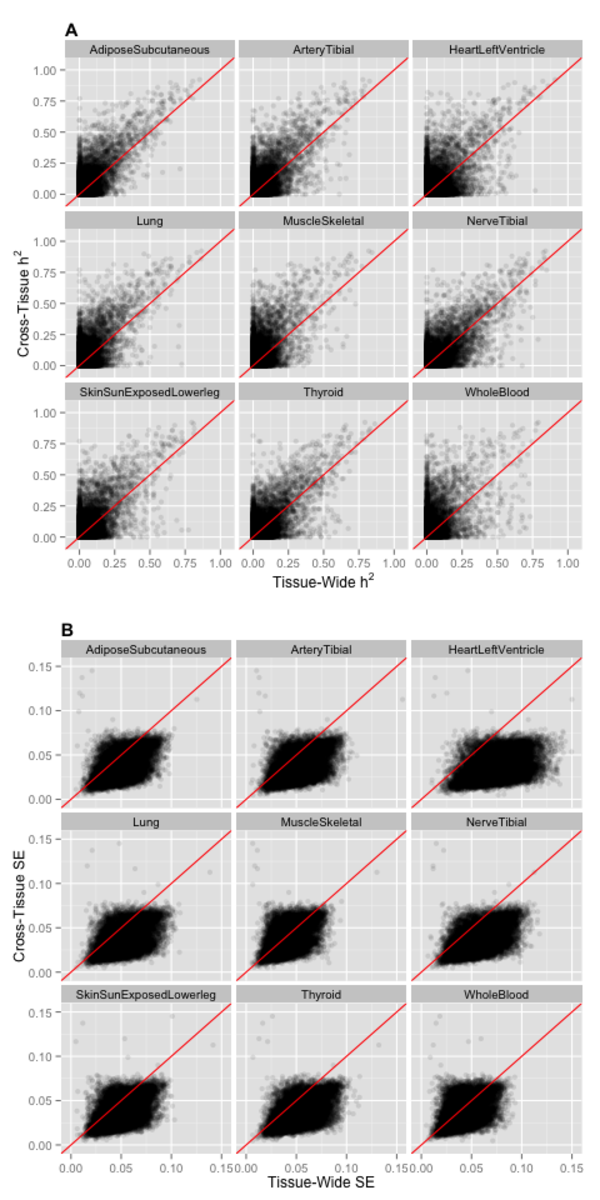
\includegraphics{GenArch_manuscript_files/figure-latex/TWotdH2SE-1.pdf}
\caption{Cross-tissue and tissue-wide comparison of heritability
(h\textsuperscript{2}, \textbf{A}) and standard error (SE, \textbf{B}).
Cross-tissue local h\textsuperscript{2} is estimated using the
cross-tissue component (random effects) of the mixed effects model for
gene expression and SNPs within 1 Mb of each gene. Tissue-wide local
h\textsuperscript{2} is estimated using the measured gene expression for
each respective tissue and SNPs within 1 Mb of each gene.}
\end{figure}

\begin{figure}[htbp]
\centering
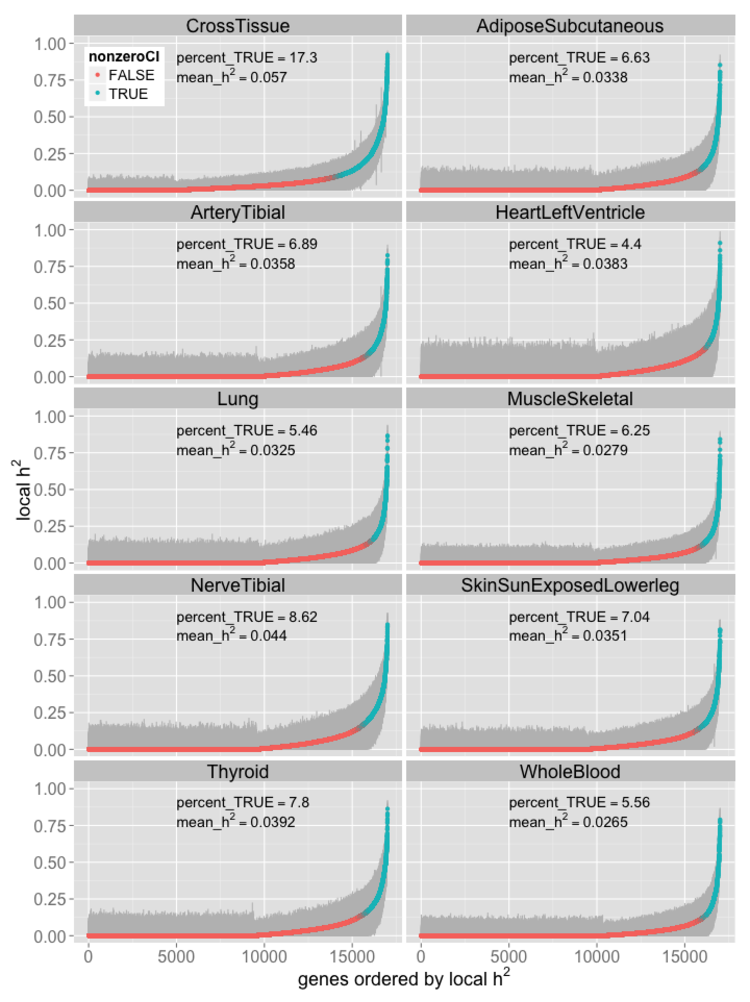
\includegraphics{GenArch_manuscript_files/figure-latex/otdTWh2-1.pdf}
\caption{Cross-tissue heritability (h\textsuperscript{2}) compared to
tissue-wide h\textsuperscript{2}. Cross-tissue local
h\textsuperscript{2} is estimated using the cross-tissue component
(random effects) of the mixed effects model for gene expression and SNPs
within 1 Mb of each gene. Tissue-wide local h\textsuperscript{2} is
estimated using the measured gene expression for each respective tissue
and SNPs within 1 Mb of each gene.}
\end{figure}

\begin{figure}[htbp]
\centering
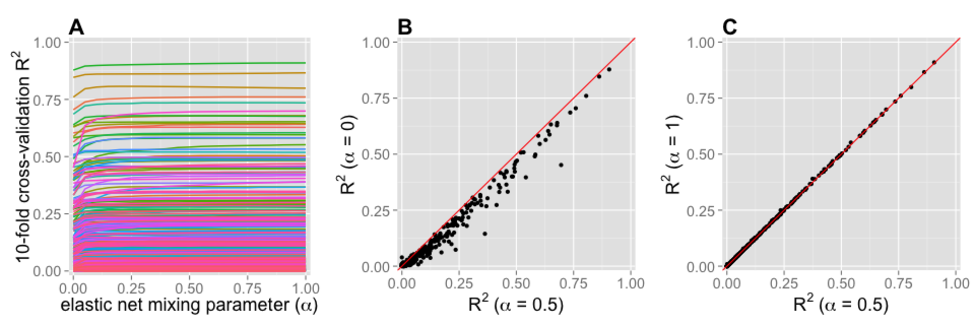
\includegraphics{GenArch_manuscript_files/figure-latex/EN-1.pdf}
\caption{Cross-validated predictive performance across the elastic net.
(\textbf{A}) 10-fold cross-validated R\textsuperscript{2} of predicted
vs.~observed expression in DGN whole blood compared to a range of
elastic net mixing parameters (\(\alpha\)) for genes on chromosome 22
with R\textsuperscript{2} \textgreater{} 0.3. (\textbf{B}) Predictive
R\textsuperscript{2} for several values of \(\alpha\) compared to
\(\alpha = 1\) (LASSO) for 341 genes on chromosome 22.}
\end{figure}

\section{Supplemental Figures}\label{supplemental-figures}

\section*{References}\label{references}
\addcontentsline{toc}{section}{References}

1. Battle A, Mostafavi S, Zhu X, Potash JB, Weissman MM, McCormick C, et
al. Characterizing the genetic basis of transcriptome diversity through
RNA-sequencing of 922 individuals. Genome Research. Cold Spring Harbor
Laboratory Press; 2013;24: 14--24.
doi:\href{http://dx.doi.org/10.1101/gr.155192.113}{10.1101/gr.155192.113}

2. Yang J, Lee SH, Goddard ME, Visscher PM. GCTA: A tool for genome-wide
complex trait analysis. The American Journal of Human Genetics. Elsevier
BV; 2011;88: 76--82.
doi:\href{http://dx.doi.org/10.1016/j.ajhg.2010.11.011}{10.1016/j.ajhg.2010.11.011}

3. Zhang X, Joehanes R, Chen BH, Huan T, Ying S, Munson PJ, et al.
Identification of common genetic variants controlling transcript isoform
variation in human whole blood. Nat Genet. Nature Publishing Group;
2015;47: 345--352.
doi:\href{http://dx.doi.org/10.1038/ng.3220}{10.1038/ng.3220}

4. Halpern BS, Regan HM, Possingham HP, McCarthy MA. Accounting for
uncertainty in marine reserve design. Ecol Letters. Wiley-Blackwell;
2006;9: 2--11.
doi:\href{http://dx.doi.org/10.1111/j.1461-0248.2005.00827.x}{10.1111/j.1461-0248.2005.00827.x}

5. Keil P, Belmaker J, Wilson AM, Unitt P, Jetz W. Downscaling of
species distribution models: A hierarchical approach. Freckleton R,
editor. Methods Ecol Evol. Wiley-Blackwell; 2012;4: 82--94.
doi:\href{http://dx.doi.org/10.1111/j.2041-210x.2012.00264.x}{10.1111/j.2041-210x.2012.00264.x}

6. R Core Team. R: A language and environment for statistical computing
{[}Internet{]}. Vienna, Austria: R Foundation for Statistical Computing;
2015. Available: \url{http://www.R-project.org/}

7. Boettiger C. Knitcitations: Citations for knitr markdown files
{[}Internet{]}. 2015. Available:
\url{http://CRAN.R-project.org/package=knitcitations}

8. Howie B, Fuchsberger C, Stephens M, Marchini J, Abecasis GR. Fast and
accurate genotype imputation in genome-wide association studies through
pre-phasing. Nat Genet. Nature Publishing Group; 2012;44: 955--959.
doi:\href{http://dx.doi.org/10.1038/ng.2354}{10.1038/ng.2354}

9. Fuchsberger C, Abecasis GR, Hinds DA. Minimac2: Faster genotype
imputation. Bioinformatics. Oxford University Press (OUP); 2014;31:
782--784.
doi:\href{http://dx.doi.org/10.1093/bioinformatics/btu704}{10.1093/bioinformatics/btu704}

\end{document}
